\textbf{Цель работы:} измерить пробег $\alpha$-частиц в воздухе двумя способами: с помощью торцевого счетчика Гейгера и синтиляционного счетчика, -- по полученным данным определить энергию частиц.
                    
\section{Теоретическое введение}

    При $\alpha$-распаде исходное родительское ядро испускает ядро гелия и превращается в дочернее ядро, число протонов и число протонов уменьшается на две единицы. Функциональная связь между энергией $\alpha$-частицы $E$ и периодом полураспада радиоактивного ядра $T_{1/2}$ хорошо описывается формулой
	\begin{equation*}
		 \lg T_{1/2} = \frac{a}{\sqrt{E}} + b.
	\end{equation*}

	Экспоненциальный характер этого процесса возникает вследствие экспоненциального затухания волновой функции в области под барьером, где потенциальная энергия больше энергии частицы.


    Экспериментально энергию $\alpha$-частиц удобно определять по величине их пробега в веществе.
	Для описания связи между энергией $\alpha$-частицы и ее пробегом пользуются эмпирическими соотношениями. В диапазоне энергий $\alpha$-частиц от $4$ до $9$ МэВ эта связь хорошо описывается выражением
	\begin{equation}
		R = 0,32 E^{3/2},
	\end{equation}
    где пробег $\alpha$-частиц в воздухе $R$ (при 15 $^\circ C$ и атмосферном давлении) выражается в сантиметрах, а энергия частицы $E$ в МэВ.

    Рассеяние $\alpha$-частиц в веществе и статистический характер потерь энергии приводят к тому, что даже при одинаковой начальной энергии пробеги разных $\alpha$-частиц несколько отличаются друг от друга. Эти различия проявляются в форме кривой, выражающей зависимость числа частиц от расстояния, пройденного ими в поглотителе.

    \begin{figure}[h!]
        \centering
        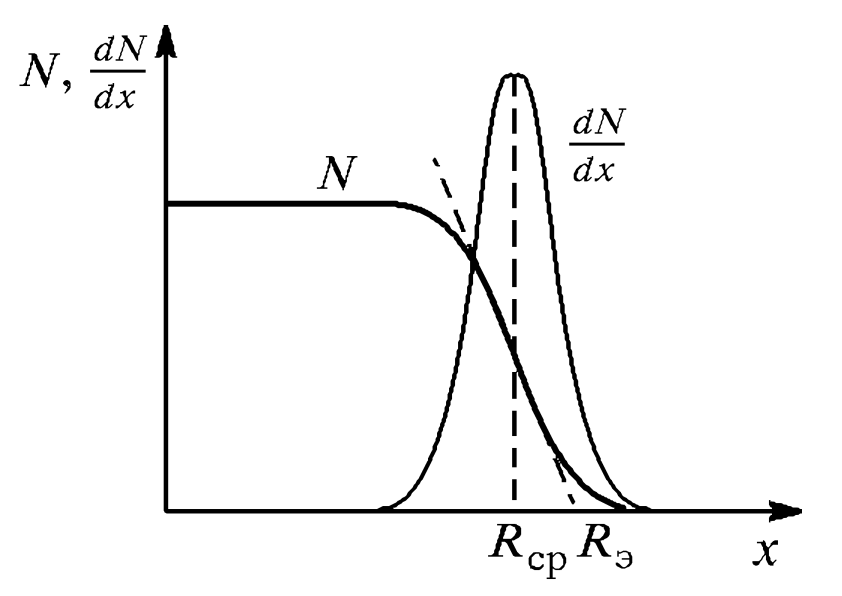
\includegraphics[width = 8.5 cm]{images/dn_dx}
        \caption{Зависимость числа $\alpha$-частиц от глубины их проникновения в вещество}
        \label{}
    \end{figure}

    При малых глубинах число частиц не меняется с расстоянием. В конце пути это число не сразу обрывается до нуля, а приближается к нему постепенно. Как видно из кривой $dN/dx$, большая часть $\alpha$-частиц останавливается в узкой области, расположенной около некоторого значения $x$, которое называется средним пробегом $R_{\text{ср}}$. Иногда вместо $R_{\text{ср}}$ измеряются экстраполированное значение $R_{\text{э}}$.

    Несмотря на наличие коллиматора, в данной работе мы имеем дело не с узкими параллельными пучками частиц, а с пучками конечных размеров, обладающими заметной угловой расходимостью. Это приводит к тому, что экспериментально наблюдаемые зависимости числа $\alpha$-частиц от глубины их проникновения качественно правильно передают появление брэгговского пика и, тем самым, относительную величину пробега частиц с разной энергией. 
    
    Однако в силу указанных причин брэгговский пик оказывается смещенным и сильно размытым.
    Поэтому лучшей оценкой пробега оказывается экстраполированный пробег.

\section{Экспериментальная установка}
\subsection{Счётчик Гейгера}

    Для определения пробега $\alpha$-частиц с помощью счетчика радиоактивный источник помещается на дно стальной цилиндрической бомбы, в которой может перемещаться торцевой счетчик Гейгера. Его чувствительный объем отделен от наружной среды тонким слюдяным
    окошком, сквозь которое могут проходить $\alpha$-частицы.


    Импульсы, возникающие в счетчике, усиливаются и регистрируются пересчетной схемой. Путь частиц в воздухе зависит от расстояния
    между источником и счетчиком. Перемещение счетчика производится путем вращения гайки, находящейся на крышке бомбы. Расстояние
    между счетчиком и препаратом измеряется по шкале, нанесенной на держатель счетчика.

    \begin{figure}[h!]
        \centering
        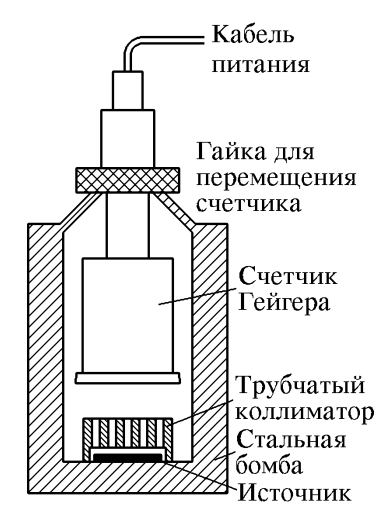
\includegraphics[width = 6 cm]{images/geiger}
        \caption{Счётчик Гейгера}
        \label{}
    \end{figure}

\subsection{Сцинтилляционный счётчик}

    Установка состоит из цилиндрической камеры, на дне которой находится исследуемый препарат. Камера герметично закрыта стеклянной пластинкой, на которую с внутренней стороны нанесен слой люминофора. С наружной стороны к стеклу прижат фотокатод фотоумножителя. Оптический контакт ФЭУ-стекло обеспечивается тонким слоем вазелинового масла.
        
    
    Сигналы с фотоумножителя через усилитель поступают на пересчетную установку. Расстояние между препаратом и люминофором составляет 9 см, так что $\alpha$-частицы не могут достигнуть люминофора при обычном давлении. Определение пробега сводится к измерению зависимости интенсивности счета от давления в камере.

    \begin{figure}[h!]
        \centering
        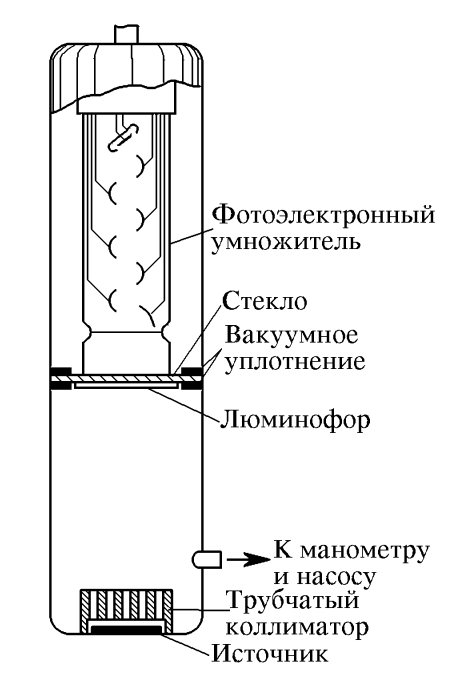
\includegraphics[width = 6 cm]{images/scint}
        \caption{Установка для измерения пробега $\alpha$-частиц с помощью сцинтилляционного счетчика}
        \label{}
    \end{figure}
    
\subsection{Иниозационная камера}

    Ионизационная камера -- прибор для количественного измерения ионизации, произведенной заряженными частицами при прохождении
    через газ. Камера представляет собой наполненный газом сосуд с двумя электродами. Сферическая стенка прибора служит одним из электродов, второй электрод вводится в газ через изолирующую пробку. К электродам подводится постоянное напряжение от источника ЭДС.
    Заполняющий сосуд газ сам по себе не проводит электрический ток, возникает он только при прохождении быстрой заряженной частицы, которая
    рождает в газе на своем пути ионы.

    Поместим на торец внутреннего электрода источник ионизирующего излучения, заполним объем камеры воздухом. Зависимость силы тока, протекающего через камеру, от приложенной разности потенциалов представлен на рисунке. Плато в зависимости объясняется отсутствием рекомбинации ионов на своём пути, то есть ионы доходят до противоположного электрода.

    Прохождение тока через камеру регистрируется посредством измерения напряжения на включенном в цепь камеры сопротивлении $R$. При изменении давления в камере ионизационный ток меняется так, как это показано на рисунке. При небольших давлениях газа $\alpha$-частицы передают часть энергии стенкам камеры. По достижении давления $P_0$ все они заканчивают свой пробег внутри газа, и дальнейшее возрастание тока прекращается. Для определения давления $P_0$ чаще всего пользуются методом экстраполяции, продолжая наклонный и горизонтальный участки кривой до пересечения. Найденный таким образом пробег затем должен быть приведен к нормальному давлению и температуре 15 $^\circ C$.

    \begin{figure}[h!]
        \centering
        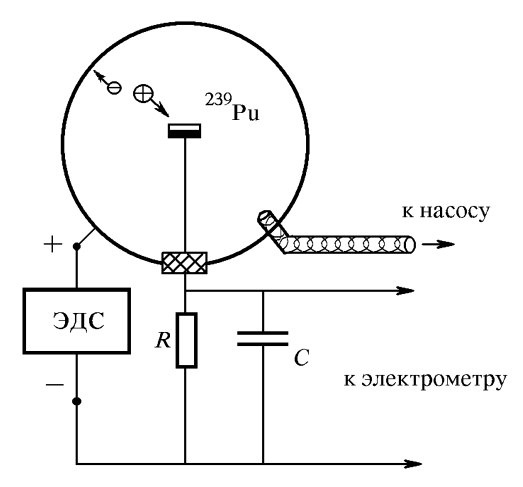
\includegraphics[width = 7 cm]{images/ion}
        \caption{Установка для измерения пробега $\alpha$-частиц с помощью ионизационной камеры}
        \label{}
    \end{figure}
    
\section{Ход работы}
\subsection{Измерение длины пробега $\alpha$-частиц с помощью счётчика Гейгера}

    Построим таблицу измеренных данных.

    \begin{table}[h!]
        \centering
        \begin{tabular}{|c|c|c|c|c|c|c|c|}
        \hline
        $x$, мм & $N_0$ & $t$, с & $N$, $\text{с}^{-1}$ & $x$, мм & $N_0$ & $t$, с & $N$, $\text{с}^{-1}$ \\ \hline
        10.00   & 149 & 10.19  & 14.626                 & 19.00   & 57  & 90.19  & 0.632                  \\ \hline
        11.00   & 519 & 30.43  & 17.057                 & 20.00   & 16  & 41.00  & 0.390                  \\ \hline
        12.00   & 638 & 40.08  & 15.918                 & 21.00   & 26  & 70.06  & 0.371                  \\ \hline
        13.00   & 685 & 45.07  & 15.199                 & 22.00   & 18  & 65.25  & 0.276                  \\ \hline
        14.00   & 600 & 40.07  & 14.972                 & 24.00   & 17  & 70.21  & 0.242                  \\ \hline
        15.00   & 430 & 30.29  & 14.197                 & 26.00   & 14  & 70.20  & 0.199                  \\ \hline
        6.00    & 646 & 45.24  & 14.280                 & 28.00   & 13  & 54.79  & 0.237                  \\ \hline
        17.00   & 605 & 49.25  & 12.284                 & 30.00   & 15  & 69.96  & 0.214                  \\ \hline
        18.00   & 217 & 40.06  & 5.416                  & --      & --  & --     & --                     \\ \hline
        \end{tabular}
        \caption{Таблица измеренных значений для счётчика Гейгера}
    \end{table}

    \begin{figure}[h!]
        \centering
        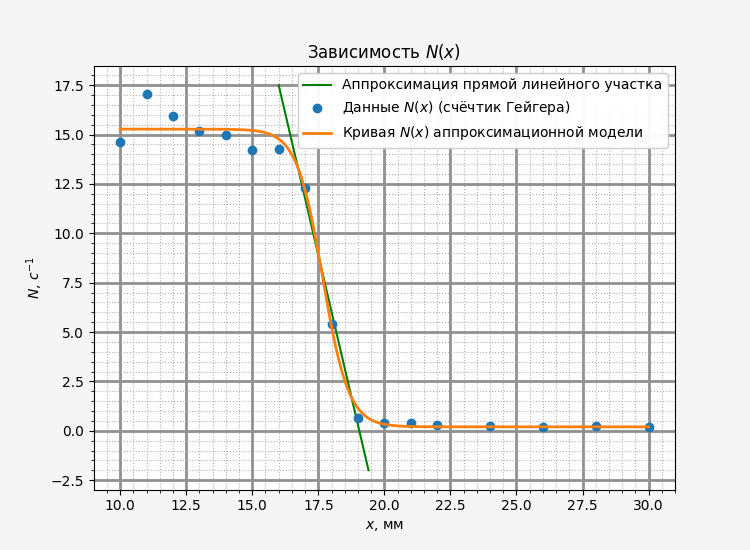
\includegraphics[width = 14 cm]{images/method_1}
        \caption{График зависимости $N(x)$}
        \label{}
    \end{figure}

    Полученный график совпадает с теоретическим. Для поиска экстраполированного значения $R_{\text{э}}$ длины свободного пробега сперва построим модель зависимости, предполагая, что она функционально описывается следующим образом:

    \begin{equation}
        N(x) = \frac{A}{1 + e^{\frac{x - x_0}{B}}} + C
    \end{equation}

    Для построенной аппроксимационной модели получены следующие значения c помощью МНК: $A = 15.079, x_0 = 17.665 \; \text{мм}, B = 0.493 \; \text{мм}, C = 0.200$. Дисперсия для модели равна $\sigma_N = 0.335 \; \text{с}^{-1}$, что означает справедливость предположенной модели.
    
    С помощью аппроксимированной аналитической кривой найдём экстрполированное значение длины свободного пробега: $R_{\text{э}} = (19 \pm 0.5)$ мм. Этой длине свободного пробега соответствует значение энергии $E = (3.27 \pm 0.13)$ МэВ. Отметим, что значение энергии занижено, так как в эксперименте используется плёнка на источнике $\alpha$-частиц.

\subsection{Измерение длины пробега $\alpha$-частиц с помощью сцинтилляционного счётчика}

    Построим таблицу измеренных данных.

    \begin{table}[h!]
        \centering
        \begin{tabular}{|c|c|c|c|c|c|c|c|}
        \hline
        $P$, торр & $N_0$  & $t$, с & $N$, $\text{с}^{-1}$ & $P$, торр & $N_0$ & $t$, с & $N$, $\text{с}^{-1}$ \\ \hline
        30        & 3936 & 10.0   & 393.600                & 210       & 550 & 15.0   & 36.667                 \\ \hline
        50        & 3471 & 10.0   & 347.100                & 230       & 269 & 15.0   & 17.933                 \\ \hline
        70        & 3060 & 10.0   & 306.000                & 250       & 165 & 15.0   & 11.000                 \\ \hline
        90        & 2730 & 10.0   & 273.000                & 270       & 203 & 25.0   & 8.120                  \\ \hline
        110       & 2376 & 10.0   & 237.600                & 290       & 96  & 25.0   & 3.840                  \\ \hline
        130       & 1973 & 10.0   & 197.300                & 310       & 3   & 25.0   & 0.120                  \\ \hline
        150       & 1431 & 10.0   & 143.100                & 330       & 0   & 25.0   & 0.000                  \\ \hline
        170       & 1004 & 10.0   & 100.400                & 350       & 0   & 25.0   & 0.000                  \\ \hline
        190       & 697  & 10.0   & 69.700                 & 370       & 0   & 25.0   & 0.000                  \\ \hline
        \end{tabular}
        \caption{Таблица измеренных значений для сцинтилляционного счётчика}
    \end{table}

    \begin{figure}[h!]
        \centering
        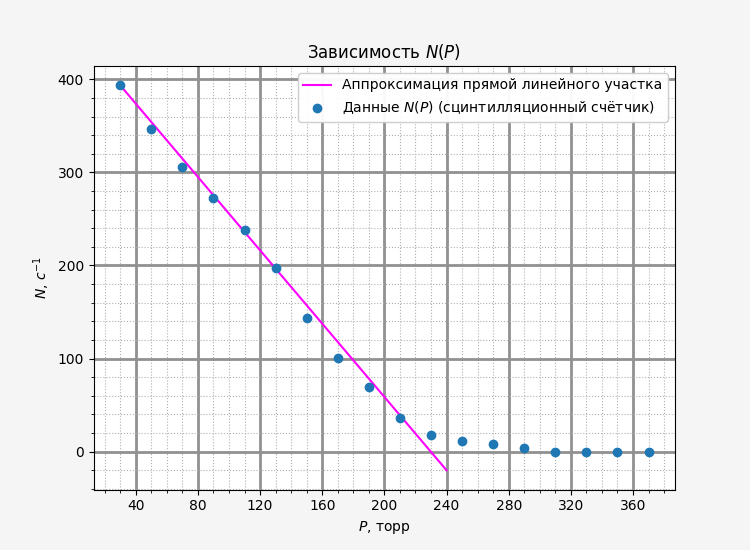
\includegraphics[width = 14 cm]{images/method_2}
        \caption{График зависимости $N(P)$}
        \label{}
    \end{figure}

    С помощью аппроксимационной прямой определим $P_{\text{э}} = (230 \pm 5)$ торр -- давление, при котором длина свободного пробега равна расстоянию от источника для люминофора $L = 9$ см. Пересчитаем длину свободного пробега для нормальных условий:
    \begin{equation}
        R_{\text{э}} = L \frac{P_{\text{э}}}{P_0}, \; P_0 = 760 \; \text{торр} \Rightarrow R_{\text{э}} = (27.2 \pm 0.8) \; \text{мм}.
    \end{equation}

    Этой длине свободного пробега соответствует значение энергии $E = (4.16 \pm 0.18)$ МэВ.

\subsection{Измерение длины пробега $\alpha$-частиц с помощью ионизационной камеры}

    Построим таблицу измеренных данных.

    \begin{table}[h!]
        \centering
        \begin{tabular}{|c|c|c|c|c|c|}
        \hline
        $P$, торр & $I$, пА & $P$, торр & $I$, пА & $P$, торр & $I$, пА \\ \hline
        37        & 37      & 260       & 426     & 520       & 967     \\ \hline
        25        & 10      & 280       & 463     & 540       & 1010    \\ \hline
        45        & 50      & 300       & 496     & 560       & 1035    \\ \hline
        65        & 80      & 320       & 540     & 580       & 1041    \\ \hline
        85        & 115     & 340       & 583     & 600       & 1045    \\ \hline
        100       & 140     & 360       & 620     & 620       & 1043    \\ \hline
        120       & 170     & 380       & 666     & 640       & 1038    \\ \hline
        140       & 206     & 400       & 708     & 660       & 1039    \\ \hline
        160       & 239     & 420       & 755     & 550       & 1006    \\ \hline
        180       & 277     & 440       & 795     & 570       & 1032    \\ \hline
        200       & 308     & 460       & 841     & 590       & 1037    \\ \hline
        220       & 351     & 480       & 887     & 610       & 1043    \\ \hline
        240       & 388     & 500       & 935     & --        & --      \\ \hline
        \end{tabular}
        \caption{Таблица измеренных значений для ионизационной камеры}
    \end{table}

    \begin{figure}[h!]
        \centering
        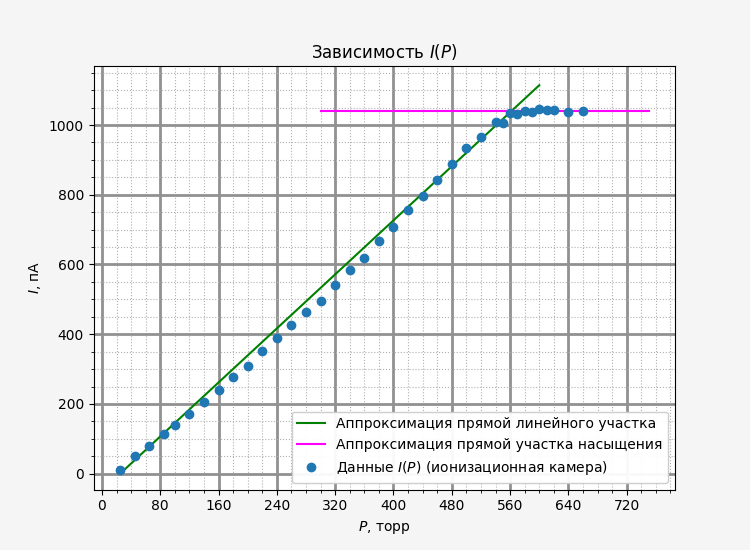
\includegraphics[width = 14 cm]{images/method_3}
        \caption{График зависимости $I(P)$}
        \label{}
    \end{figure}

    С помощью аппроксимационной прямой определим $P_{\text{э}} = (560 \pm 5)$ торр -- давление, при котором длина свободного пробега равна расстоянию между внутренним и внешним электродами $L = (10 - 0.5) / 2 = 4.75$ см ($10$ см -- диаметр внешнего диска, $0.5$ см -- внутреннего). Пересчитаем длину свободного пробега для нормальных условий:
    \begin{equation}
        R_{\text{э}} = L \frac{P_{\text{э}}}{P_0}, \; P_0 = 760 \; \text{торр} \Rightarrow R_{\text{э}} = (28.8 \pm 0.3) \; \text{мм}.
    \end{equation}

    Этой длине свободного пробега соответствует значение энергии $E = (4.33 \pm 0.07)$ МэВ.

\section{Заключение}

    Тремя различными способами был измерен свободный пробег в воздухе $\alpha$-частиц с энергией 5,15 МэВ. В качестве источника радиоактивных частиц был использован $^{239}$Pu.

    В результате экспериментов были получены следующие значения энергии $\alpha$-частиц: с помощью счётчика Гейгера $E = (3.27 \pm 0.13)$ МэВ, с помощью сцинтилляционного счётчика $E = (4.16 \pm 0.18)$ МэВ, с помощью ионизационной камеры $E = (4.33 \pm 0.07)$ МэВ.

    Полученные значения является заниженными по сравнению с теоретическим по следующим причинам: источник частиц покрыт слюдяной пленкой, что приводит к замедлению $\alpha$-частиц; пучки частиц обладают конечными размерами, что приводит к угловой расходимости и заметно искажает брэгговский пик, из-за чего зависимости являются более размытыми.

